\documentclass[12pt,a4paper]{report}
\usepackage[pdftex]{graphicx}
\usepackage{fontspec}
\usepackage{inconsolata}
\usepackage{subcaption}
\usepackage{listings}
\usepackage[dvipsnames]{xcolor}
\usepackage{url}
\usepackage[bookmarks, colorlinks=false, pdfborder={0 0 0}, urlcolor=cyan, citecolor=black, anchorcolor=black]{hyperref} 

\lstset{
    basicstyle=\fontsize{8}{10}\selectfont\ttfamily,
    tabsize=4,
    keywordstyle=\color{blue}\selectfont\ttfamily,
    stringstyle=\color{BrickRed}\selectfont\ttfamily,
    commentstyle=\color{ForestGreen}\selectfont\ttfamily,
    showstringspaces=false,
    showtabs=false,
}


\begin{document}

\renewcommand\bibname{Quellenverzeichnis} 
\renewcommand{\contentsname}{Inhalt}
\renewcommand{\listfigurename}{Abbildungsverzeichnis}
\renewcommand{\chaptername}{Kapitel}
\renewcommand{\figurename}{Abbildung}


\begin{titlepage}

\begin{center}

\textup{\small {\bf Projektarbeit Systemadministration} \\ Dokumentation}\\[0.2in]

% Title
\Large \textbf {Automatische Eintritts\"uberwachung an Geb\"aude-Zug\"angen}\\[0.5in]

        \small{Studiengang Angewandte Informatik}\\
        \vspace{.2in}
       \normalsize{16. Dezember 2016}
       \vspace{.4in}

\begin{table}[h]
\centering
\begin{tabular}{ll} \\
Matrikel Nr. & Name des Autors \\ \\ \hline
\\
24634 & Markus Birkler \\
24637 & Daniel Schukies \\ \\ \hline
\end{tabular}
\end{table}

\vspace{.1in}
Unter der Leitung von\\
{\textbf{Prof. Dr. Tobias Eggendorfer}}\\[0.2in]

\vfill


\includegraphics[width=0.5\textwidth]{hs}\\[0.2in]
\Large{Fakult\"at f\"ur Elektrotechnik und Informatik}\\
\normalsize
\textsc{Hochschule Ravensburg-Weingarten}\\
Weingarten, Baden-W\"urttemberg, Deutschland \\
\vspace{0.2cm}
Wintersemester 2016

\end{center}

\end{titlepage}

\newpage
\thispagestyle{empty}

\begin{center}

\emph{\LARGE Ehrenw\"ortliche Erkl\"arung}\\[2.5cm]
\end{center}
\normalsize Wir versichern hiermit, dass wir die vorliegende Arbeit selbst\"andig angefertigt, alle Hilfen und Hilfsmittel angegeben und alle Fremdinhalte, einschlie{\ss}lich dem Internet entnommene Inhalte kenntlich gemacht haben. \\[1.0cm]

\begin{table}[h]
\begin{tabular}{lr}
\hline
\\
24634 & Markus Birkler \\ 
24637 & Daniel Schukies \\
\end{tabular}
\end{table}

\vfill

\begin{flushleft}
Weingarten, den 16. Dezember 2016
\end{flushleft}

\pagenumbering{roman} 
\tableofcontents

\newpage
\pagenumbering{arabic} 

\chapter{Einleitung}

\section{Motivation}
\"Ublicherweise nehmen \"Uberwachungssysteme den betreffenden Bereich von 24 Stunden am Tag auf. Das erzeugt eine Menge \"Uberwachungsmaterial, in dem man schnell die \"Ubersicht verliert und unn\"otig viel Speicherkapazit\"at verbraucht.\\
\\
Wenn eine kontinuierliche Aufzeichnung eines Bereichs nicht erforderlich ist, kann der \"Uberwachungsprozess durch "on-demand"-Betrieb der Anlage optimiert werden. 
Die Grundidee hinder dem Projekt ist, einen Geb\"aude-Zugang nur dann aktiv zu \"uberwachen, wenn er genutzt wird (i.e. wenn die T\"ur ge\"offnet wird).
\\

\section{Ziele}
Erstellt werden soll ein System zur automatischen Eintritts\"uberwachung an Geb\"aude-Zug\"angen.\\
\\
Das System soll vollst\"andig autonom Video-Aufnahmen von Personen machen, welche den vom System \"uberwachten Zugang nutzen.
Zu diesem Zweck wird ein Raspberry Pi mit Kamera und Magnetschalter ausgestattet. \\
\\
Der Magnetschalter wird an der T\"ur des zu \"uberwachenden Zugangs positioniert, sodass  er \"offnet/schlie{\ss}t, wenn die T\"ur ge\"offnet/geschlossen wird.
Die Kamera wird mit Blickrichtung zur T\"ur positioniert, um sp\"ater im Video das Gesicht der Person erkennen zu k\"onnen.\\
\\
Sobald nun der Magnetschalter das \"Offnen der T\"ur meldet, beginnt die Aufzeichnung des \"Uberwachungs-Videos \"uber die Kamera. Die Aufzeichnung wird fortgesetzt soange die T\"ur offen bleibt. Wird die T\"ur geschlossen, wird die Aufnahme nach einigen Sekunden beendet.\\
Durch die Verz\"ogerung des Aufnahme-Stopps soll sichergestellt werden, dass im Fall einer Manipulation des Magnetschalters (z.B. mit K\"uhlschrank-Magnet) immer noch ausreichend \"Uberwachungsmaterial gesammelt wird.\\
\\
Alle Aktivit\"aten werden mit Zeitstempel und Verweis auf die Video-Dateien in der Datenbank des Raspberry Pi hinterlegt.
\"Uber ein im lokalen Netz erreichbares Webinterface k\"onnen Zugangszeiten und die damit assoziierten Aufzeichnungen eingesehen/heruntergeladen werden.\\
Videomaterial \"alter als der konfigurierte Zeitraum wird gel\"oscht.\\
\\
Das System ist nicht als Alarmanlage oder Schutzma{\ss}nahme gegen Einbruch zu verstehen.
\\

\section{Eigene Leistung}
Die eigene Leistung umfasst neben der schriftlichen Ausarbeitung die Erstellung eines Prototyps mithilfe der ausgew\"ahlten Hardware und Software als Beweis f\"ur die Realiserbarkeit der Projektidee.

\newpage

\section{Gantt-Diagramm}

\begin{figure}[ht]
    \centering
    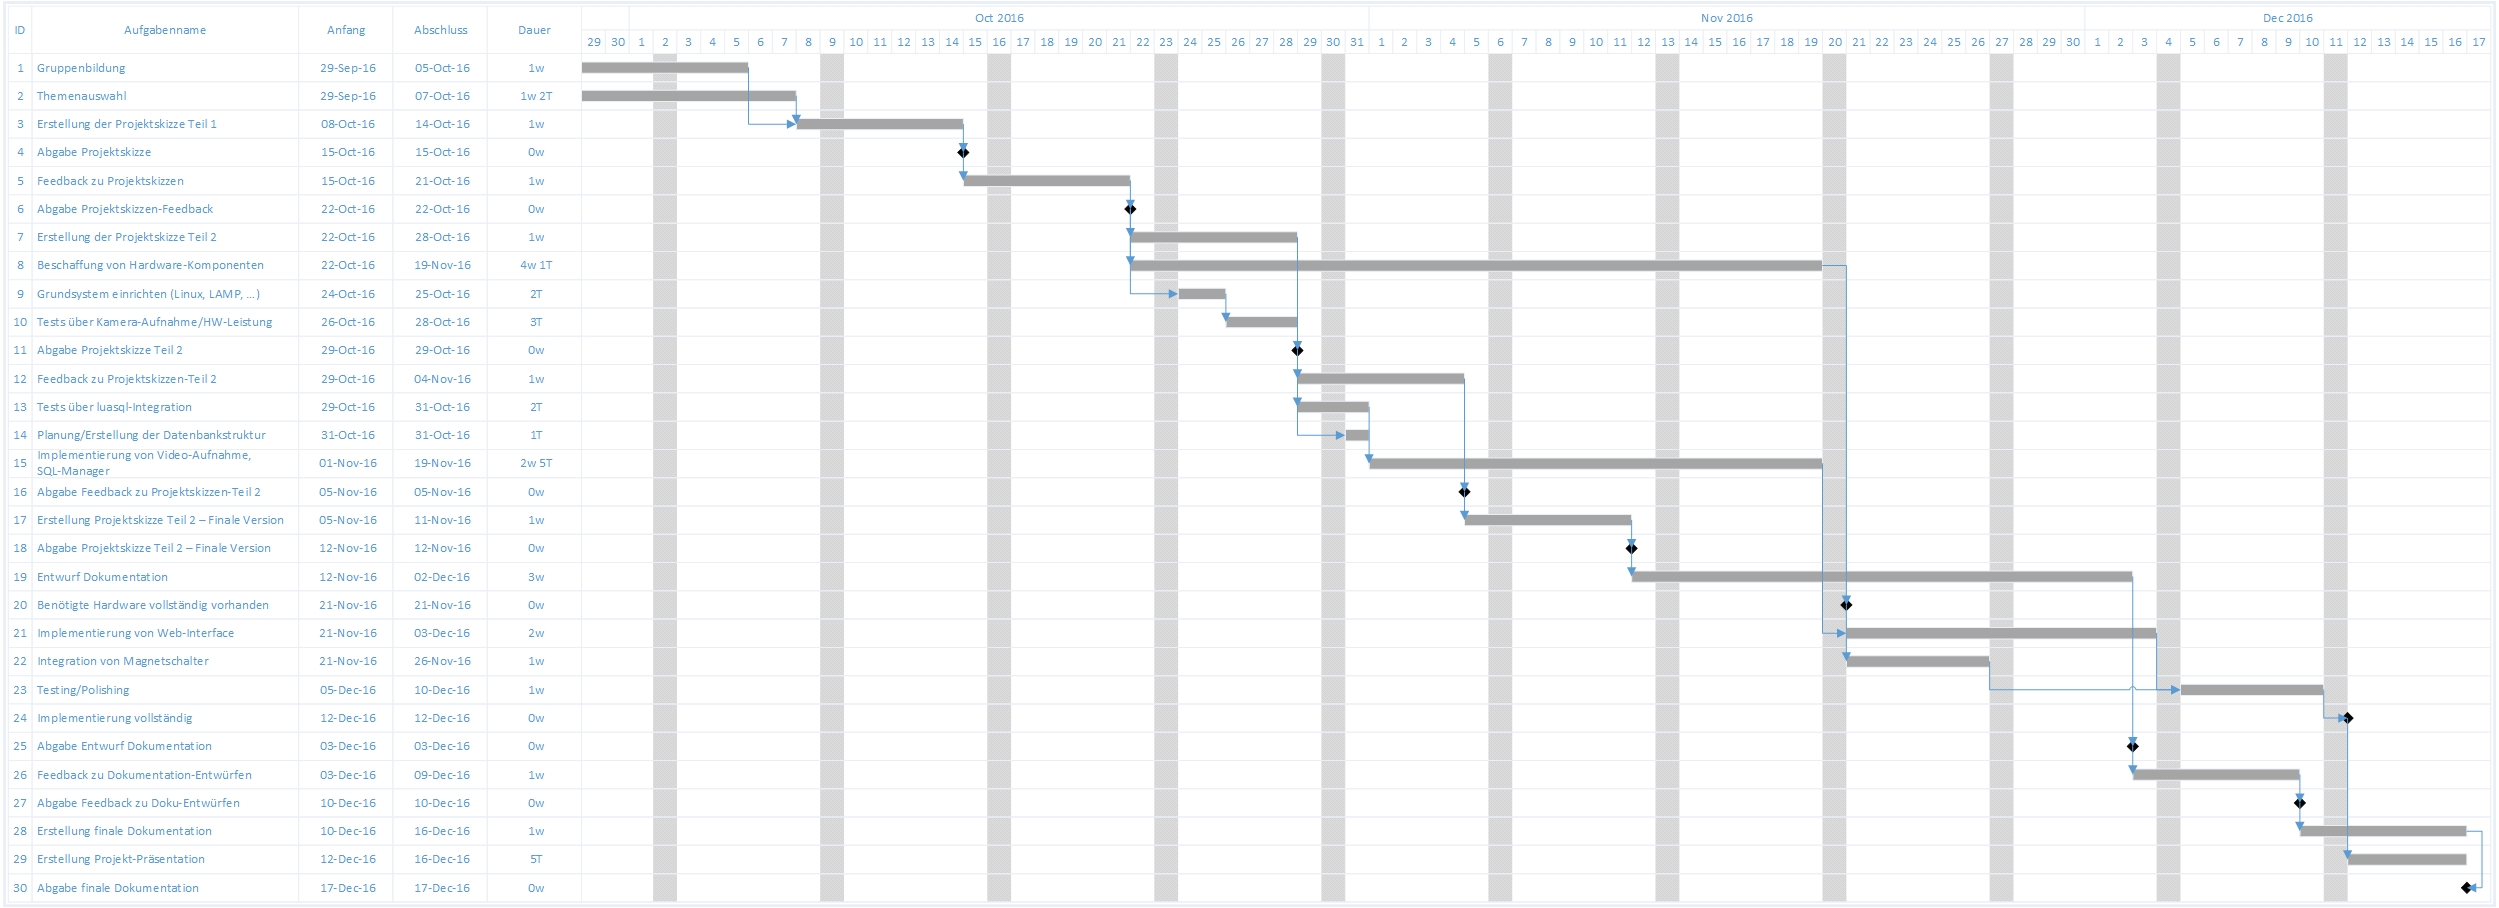
\includegraphics[angle=90,scale=0.3]{images/gantt}
    %\caption{Gantt-Diagramm}
    \label{fig:gantt}
\end{figure}

\newpage 
\chapter{Grundlagen}

\section{Raspberry Pi}
Der Raspberry Pi ist ein Einplatinencomputer im Smartcard-Format. Er ist dank seiner geringen Größe sehr komfortabel platzierbar und benötigt keine weiteren Montage-Maßnahmen. Der Raspberry Pi ist sehr beliebt für experimentelle Projekte.\\
\\
Die Dokumentation des Raspberry Pi sowie Community-Inhalte sind verfügbar unter \href{https://www.raspberrypi.org/}{https://www.raspberrypi.org/}
\vspace{1.0cm}

\section{GPIO}
GPIO (\textbf{G}eneral \textbf{P}urpose \textbf{I}nput/\textbf{O}utput) ist eine Schnittstelle, deren Verhalten durch Programmierung frei bestimmt werden kann. Es können einzelne Pins wahlweise als Eingang(zum Lesen) oder Ausgang( High- oder Low- Signal) definiert werden. Ist ein Pin als Eingang konfiguriert, und es liegt kein Signal an, befindet sich der Eingang in einem hochohmigen Zustand(Tri-State). Das bedeutet, dass der Eingang weder High noch Low ist. Die Pegelspannung beim Raspberry Pi beträgt ungefähr +1V (Low)\footnote{Erfahrungswert} und +3.3V (High).
\vspace{1.0cm}

\section{Reed-Kontakt}
Reed-Kontakte (Reed-Relais) sind ferromagnetische Sensoren, die in Anwesenheit eines Magnetfelds einen elektrischen Strom schalten.\\
Diese Art won Sensorik eignet sich gut zur Erkennung mechanischer Prozesse (wie beispielsweise das Öffnen einer Tür).
\vspace{1.0cm}

\section{Apache HTTPD}
Der Apache HTTP Server ist der open-source Webserver der Apache Software Foundation. Der Server ist durch viele Module in seiner Funktion erweiterbar.\\
\\
Das Projekt ist unter \url{https://httpd.apache.org} gehostet.
\vspace{1.0cm}

\section{PHP}
PHP ist eine serverseitige Skriptsprache zur Generierung von dynamischen Webinhalten. Über PHP können zum Beispiel Einträge aus  Datenbanken gelesen und in Websites eingebunden werden. Außerdem kann mit PHP objektorientiert programmiert werden.\\
\\
Dokumentation und weitere Informationen sind auf der Projektseite (\url{https://secure.php.net}) verfügbar.
\vspace{1.0cm}



\section{MariaDB/MySQL}
MySQL\footnote{\url{https://www.mysql.com}} ist ein open-source Datenbanksystem, das von der Oracle Corporation sowohl unter der GPL\footnote{General Public License, \url{https://www.gnu.org/licenses/gpl.html}}, als auch kommerziell lizenziert erhältlich ist.\\
Ein Fork von MySQL ist MariaDB, der als Datenbank-Kern die Speicher-Engine \textit{Aria} verwendet. Die Vorteile dieser Engine sind unter anderem erhöhte Stabilität und Geschwindigkeit\footnote{\url{https://mariadb.com/resources/blog/why-should-you-migrate-mysql-mariadb}}.\\
\\
Die Projektseite ist \url{https://mariadb.org}
\vspace{1.0cm}


\section{Lua}
Für den Großteil der Programm-Implementierung wird Lua\footnote{\url{https://www.lua.org/}} verwendet.
Lua ist eine platformunabhängige Skriptsprache, deren Installation üblicherweise nur einen schlanken Interpreter mitbringt. Wegen der hohen Performance, der geringen Installationsgröße und dem modularen Aufbau wird Lua oft im Embedded-Umfeld mit begrenzten Ressourcen eingesetzt.
\vspace{1.0cm}

\section{systemd}
systemd (system daemon) ist ein Programm zur Service-Verwaltung auf Linux-Systemen, welches als init-Prozess (PID 1) gestartet wird und weitere Hintergrundprozesse verwaltet. Es löst damit das alte SysVinit\footnote{\url{https://savannah.nongnu.org/projects/sysvinit}}-System ab. Einige große Distributionen wie Debian und Arch Linux haben systemd standardmäßig integriert.\\
\\
systemd auf freedesktop.org: \url{https://wiki.freedesktop.org/www/Software/systemd}
\newpage


\chapter{Anforderungsanalyse}

\section{Priorisierung}

\subsection{Muss}
\begin{itemize}
    \item Der Zustand der T\"ur (Offen/Zu) wird von einem Magnetschalter erfasst, welcher \"uber die GPIO-Schnitstelle mit dem Raspberry Pi verbunden ist.
    \item Die Kamera ist \"uber USB mit dem Raspberry Pi verbunden.
    \item Das System kann per WLAN \"uber einen USB-Adapter mit dem Netzwerk verbunden werden, um Installationen ohne Ehternet-Schnittstelle zu erm\"oglichen.
    \item Die Kamera muss so positioniert werden, dass das Gesicht der Person, die durch die T\"ur tritt, erkennbar ist.
    \item Die Kabel m\"ussen lang genug sein, um das System auch an gr\"o{\ss}eren Zug\"angen installieren zu k\"onnen.
    \item Auf der Hardware muss ein LAMP-Server sowie ein Datenbank-Server lauff\"ahig sein.
\end{itemize}

\subsection{Soll}
\begin{itemize}
    \item Magnet und Magnetschalter m\"ussen so an der T\"ur anbringbar sein, dass man den Mechanismus nicht umgehen kann.
    \item Das System soll stabil genug laufen, um im Dauermodus betrieben werden zu k\"onnen.
    \item Der Datenbank-Eintrag soll zu Beginn der Aufnahme geschrieben werden, damit wenigstens die Zeiterfassung funktioniert (falls Kamera ausf\"allt).
    \item Ein systemd-Service startet das Script zum Systemstart und initialisiert die Hardware.
    \item Ein systemd-Timer durchsucht im definierten Zeit-Intervall die Datenbank nach Eintr\"agen, die die definierte Speicherungszeit \"uberschritten haben, und entfernt die Video-Dateien. Die Datenbank-Eintr\"age bleiben bestehen; diese werden \"uber das Web-Interface gel\"oscht.
    \item Button zum L\"oschen aller alten Logeintr\"age in der Datenbank.
\end{itemize}

\subsection{Kann}
\label{sec:kann}
\begin{itemize}
    \item Aktivierung des Systems durch T\"urklingel
    \item Platzierung der Kamera auf Motorplatte zur Erweiterung des \"Uberwachungsbreichs
    \item Unterst\"utzung f\"ur dedizierte Datenbank-Server/Videospeicher
    \item Ton-Aufzeichnung
    \item Gesichtserkennung von eingehenden Personen
    \item Live-Stream der Kamera \"uber Web-Interface
\end{itemize}

\newpage
\chapter{Marktanalyse}
\section{Existierende L\"osungen}

\begin{description}
   \begin{itemize}
    \item \href{http://www.forum-raspberrypi.de/Thread-funk-magnetkontakt-reed-switch-zur-fenster-tuer-ueberwachung-tinytx3}{Alarmanlage – Kabellose Überwachung von Fenstern und Türen mit dem Raspberry Pi}
    \item \href{http://www.forum-raspberrypi.de/Thread-tutorial-alarmanlage-magnetkontakte-auslesen-und-speichern-webserver-interface}{Alarmanlage - Magnetkontakte auslesen und speichern - Webserver Interface}
    \item Kommerzielle Lösungen
   \end{itemize}
\end{description}

\section{Bewertung}

Für die Marktanalyse wurden 10 ähnliche Lösungen gesucht und mit diesem Projekt verglichen.
Dabei handelt es sich um zwei Projekte mit dem Raspberry PI und kommerzielle Lösungen mit anderer Hardware.

\paragraph {Kabellose Überwachung von Fenstern und Türen mit der Raspberry Pi} 

Aufwendige konstruktion durch die Funklösung. Bietet keine aufzeichnung von Videos.

\paragraph {Alarmanlage - Magnetkontakte auslesen und speichern - Webserver Interface} 

Diese Lösung funktioniert ebenfalls mit einem Raspberry PI und einem Magnetsensor. Es stellt ein Webinterface zur Verfügung, bietet aber keine automatische aufzeichnung von Videos.

\paragraph {Kommerzielle Lösungen}

Haben Vergleichsweise hohe Anschaffungskosten. Die gefundenen Lösungen bieten die Aufzeichnung von Videos mittels Bewegungserkennung an einer IP-Camera\footnote{\href{https://en.wikipedia.org/wiki/IP_camera}{https://en.wikipedia.org/wiki/IP_camera}}.
\chapter{Implementierung}

\section{Hardware}
\subsection{Raspberry Pi}

\begin{figure}[ht]
    \centering
    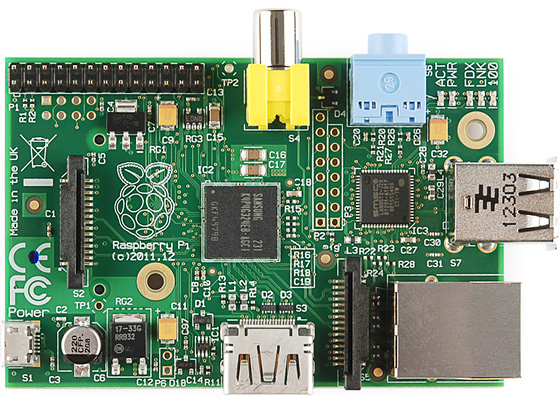
\includegraphics[scale=0.3]{images/raspberrypi}
    \caption{ \cite{img01} Raspberry Pi Modell B (oben)}
    \label{fig:raspberrypi}
\end{figure}
Das ausgew\"ahlte Modell B besitzt u.a. einen 700MHz Broadcom-Prozessor (ARM-Architektur), 500MB Arbeitsspeicher, 2 USB-2.0-Anschl\"usse sowie 17 frei programmierbare GPIO-Pins.
Auf dem Raspberry Pi wird Debian GNU/Linux einngesetzt.

\newpage

\subsection{Kamera}

\begin{figure}[ht]
    \centering
    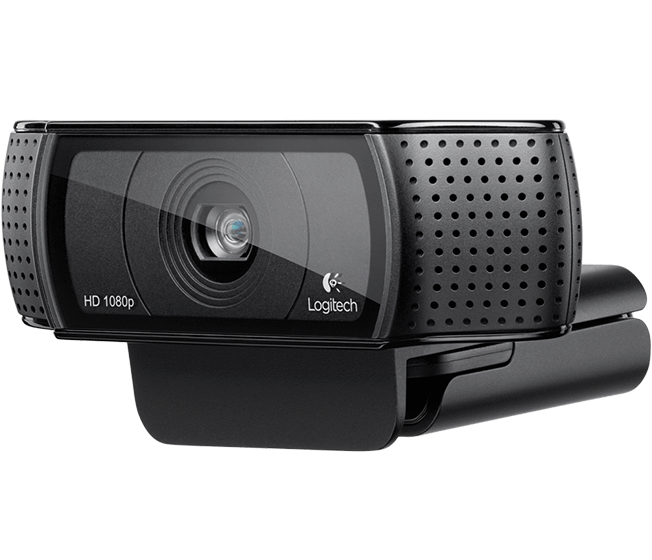
\includegraphics[scale=0.2]{images/c920webcam}
    \caption{\cite{img02} Logitech HD Pro Webcam C920}
    \label{fig:webcam}
\end{figure}
Als Kamera wird eine Logitech HD Pro Webcam C920 verwendet\footnote{\href{https://secure.logitech.com/en-us/product/hd-pro-webcam-c920}{https://secure.logitech.com/en-us/product/hd-pro-webcam-c920}}.
Die USB-Kamera unterst\"utzt Aufnahmen mit bis zu 1920x1080 Pixel bei 30 Bildern pro Sekunde bzw. 1280x720 Pixel bei 60 Bildern pro Sekunde. Integriert ist au{\ss}erdem ein H264-Hardware-Encoder, was bei diesem Projekt besonders von Vorteil ist, da die Rechenleistung des ausgew\"ahlten Raspberry Pi-Modells nicht ausreicht, um die Video-Daten effizient zu codieren.\\


\subsection{Netzteil}
Die \"ublichen 1200mA-Netzteile sind zu schwach, wenn eine Webcam angeschlossen werden soll, da diese zeitweise eventuell einen hohen Stromverbrauch hat.
\begin{figure}[h]
    \centering
    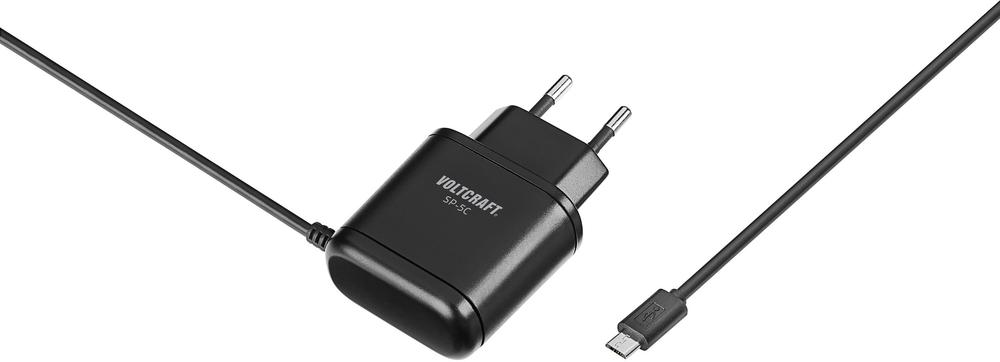
\includegraphics[scale=0.2]{images/netzteil}
    \caption{\cite{img03} Voltcraft SP-5C}
    \label{fig:netzteil}
\end{figure}
Daher wird f\"ur diesen Anwendungsfall ein \"uberlastungsgesch\"utztes 2500mA-USB-Netzteil\footnote{Das verwendete Netzteil ist ein Voltcraft SP-5C} verwendet.\\

\subsection{Sensor}
Der Sensor wird zur Erkennung des Zustands der T\"ur eingesetzt.
\begin{figure}[h]
    \centering
    \begin{subfigure}[t]{0.5\textwidth}
        \centering
        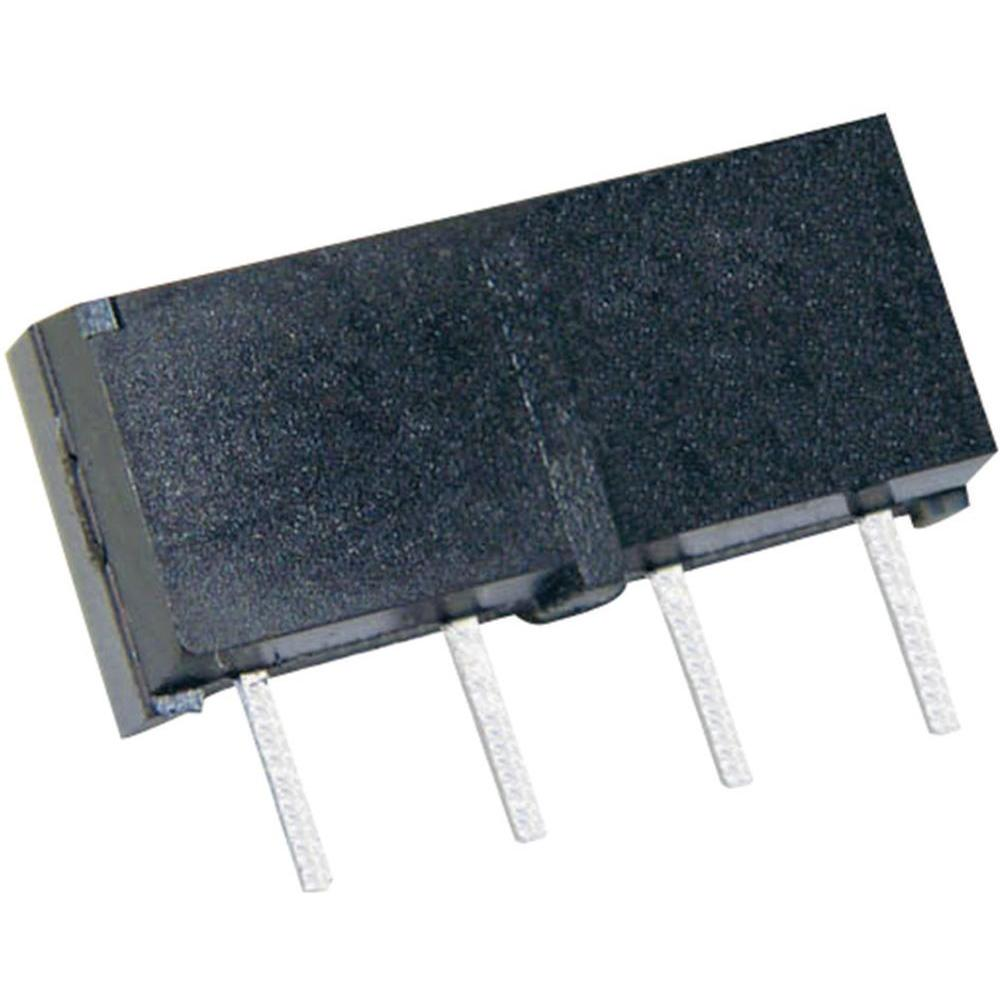
\includegraphics[scale=0.05]{images/sensor}
        \caption{\cite{img04} Reed-Kontakt}
    \end{subfigure}%
    \begin{subfigure}[t]{0.5\textwidth}
        \centering
        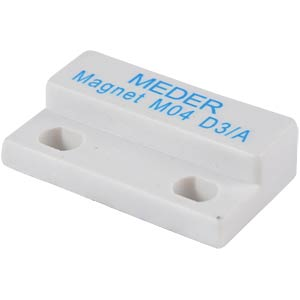
\includegraphics[scale=0.2]{images/MAGNET_M4}
        \caption{\cite{img05} Bet\"atigungsmagnet}
    \end{subfigure}
    \caption{Sensor und Magnet}
    \label{fig:sensor}
\end{figure}
\\Verwendet wird hier ein Reed-Kontakt\footnote{Genaue Bezeichnung des Bauteils: MS05-1A87-75DHR} mit passendem Bet\"atigungsmagnet.
Damit der Sensor besser befestigt werden kann wird er auf eine kupferbeschichtete Hartpapier-Platine gel\"otet. Au{\ss}erdem werden die Anschl\"usse auf eine Stiftleiste gef\"uhrt, um die Verbindung mit den GPIO-Pins des Raspberry Pi zu vereinfachen.\\

\subsection{Gesamtaufbau}
\begin{figure}[ht]
    \centering
    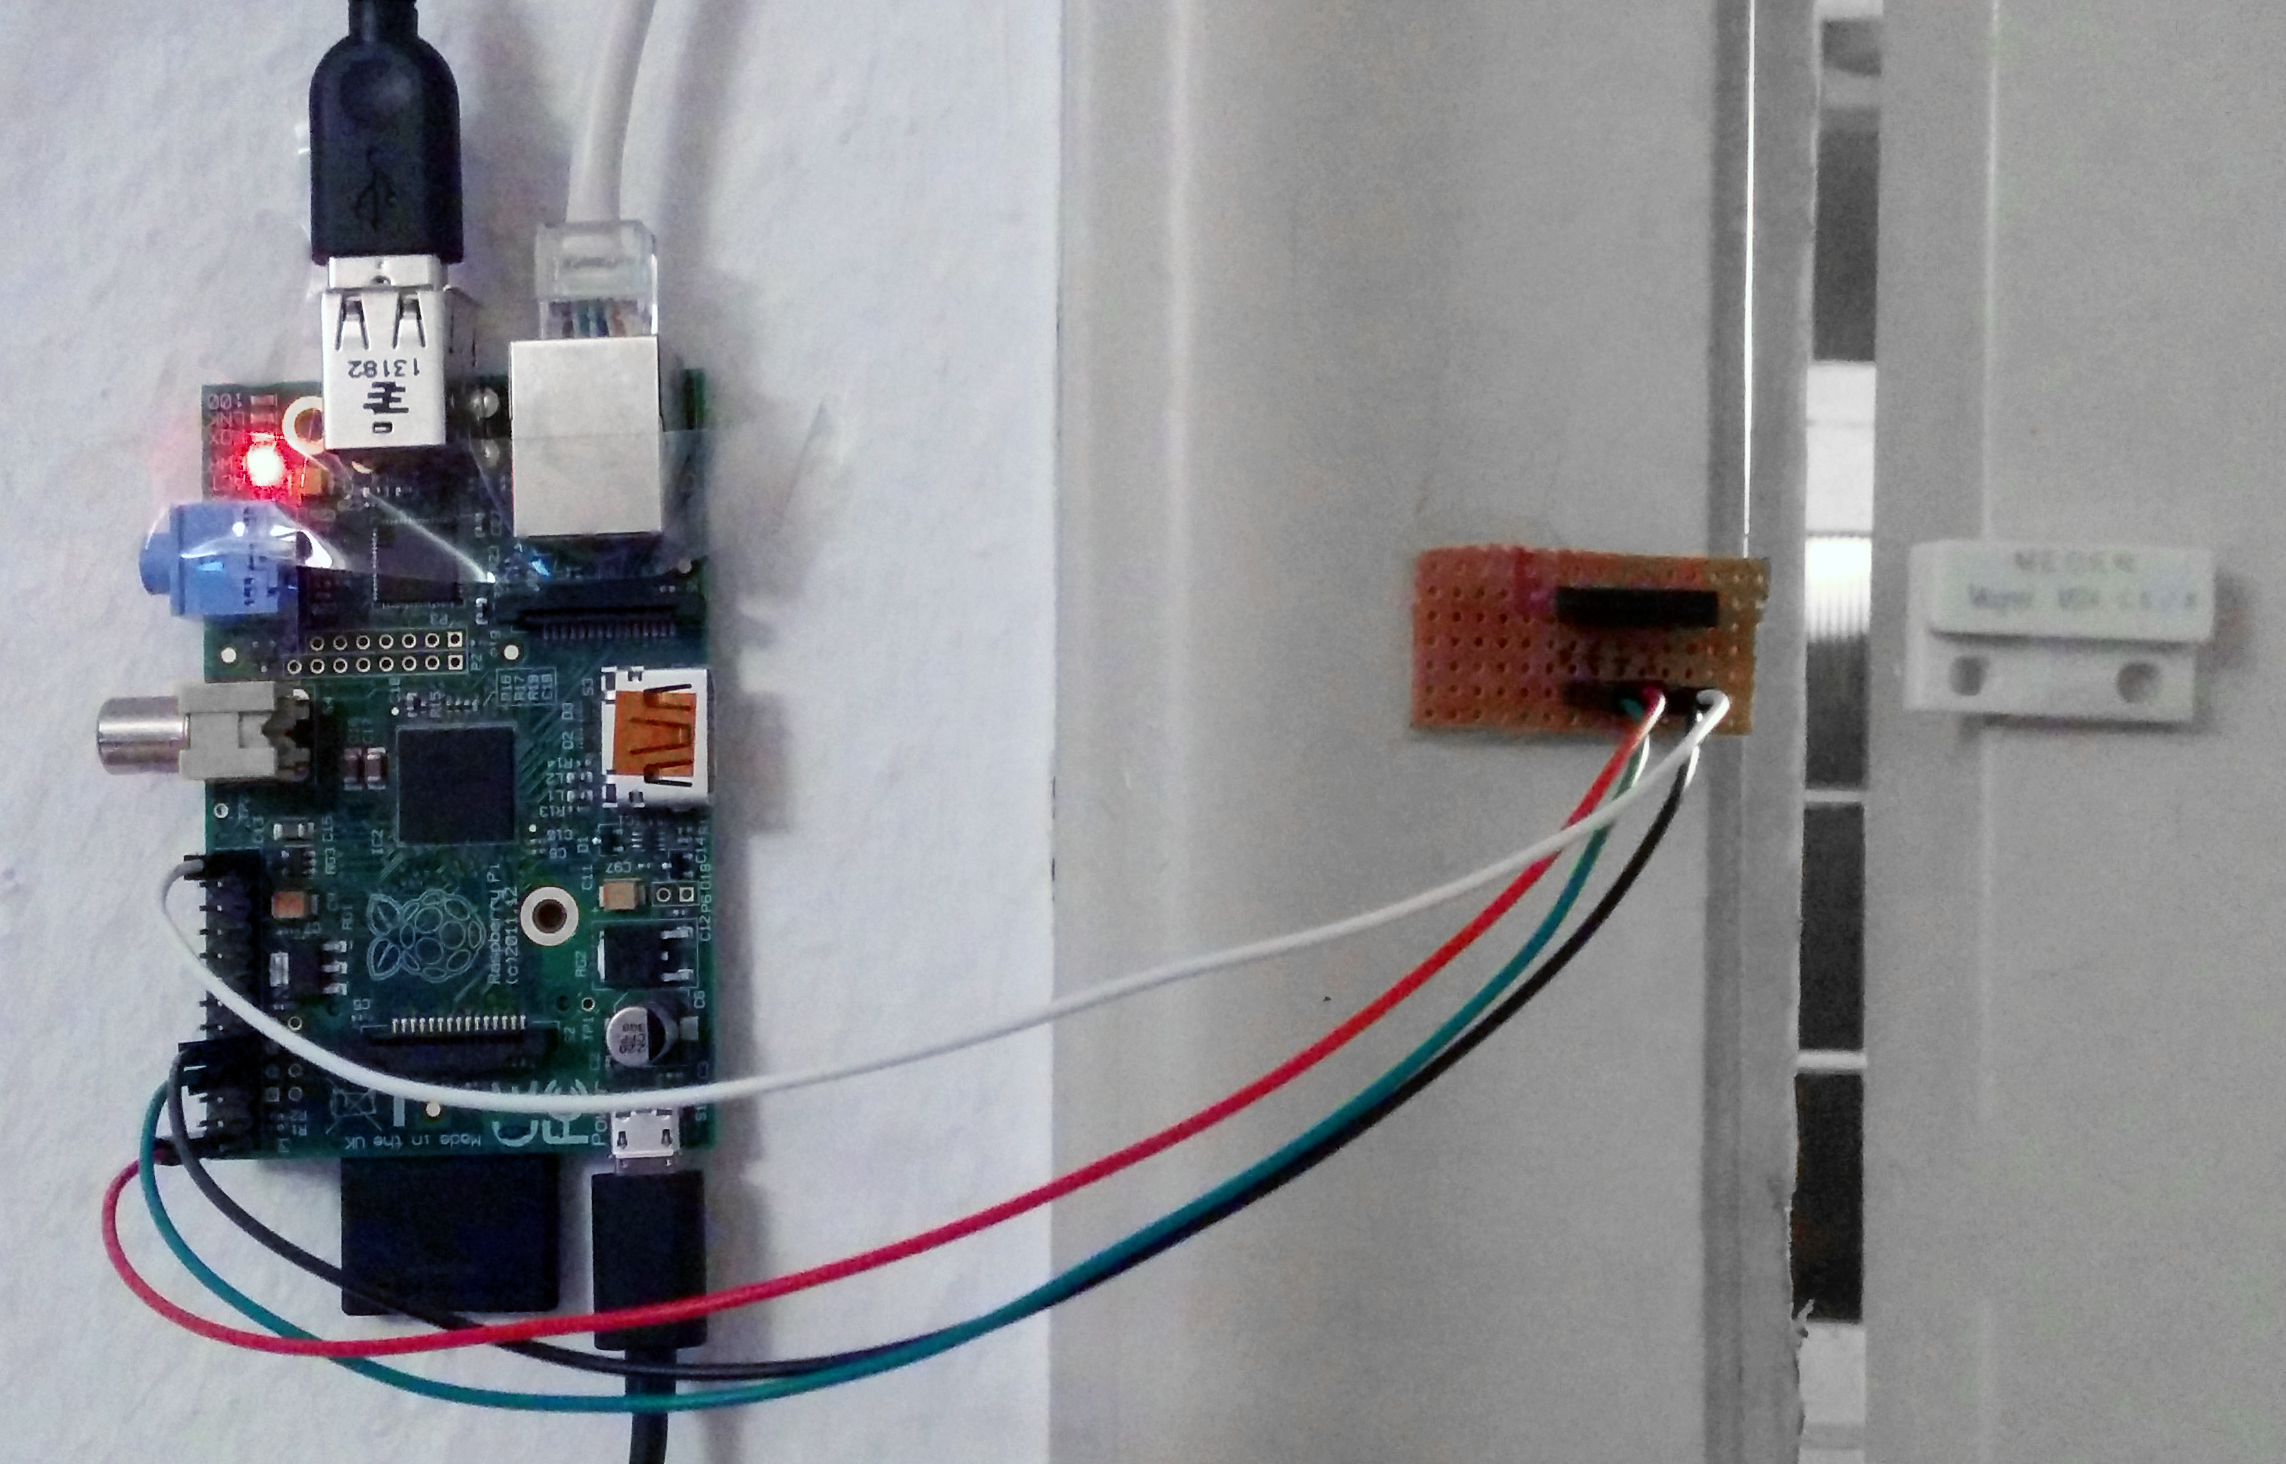
\includegraphics[scale=0.15]{images/aufbauklein}
    \caption{Gesamtaufbau der Hardware}
    \label{fig:gesamt}
\end{figure}

\newpage


\section{Software}

\subsection{Installation ben\"otigter Software}
\subsubsection{LAMP}
F\"ur das Web-Interface wird ein LAMP\footnote{LAMP(Linux-Apache-MySQL-PHP) ist ein gängiges Server-Setup}-Server ben\"otigt.\\
Installiert werden:
\begin{itemize}
    \item Apache HTTP Server Version 2.4
    \item PHP 5.6.28
    \item MariaDB Server 10.0
\end{itemize}
\vspace{0.5cm}
\subsubsection{VLC Media Player}
Der VLC Media Player\footnote{Projektseite: \url{https://www.videolan.org/vlc/}} bietet eine komfortable M\"oglichkeit, Video-Ger\"ate \"uber den Video4Linux-Treiber (V4L) anzusprechen und deren Video-Stream in einem Video-Container zu speichern. Installiert wird nur das Kommandozeilen-Frontend - die grafische Oberfl\"ache wird nicht ben\"otigt.
\\
\subsubsection{Lua}
Installiert wird aus Kompatibilit\"atsgr\"unden Lua 5.1\footnote{Aktuelle Version ist 5.3, Debian-Repository-Version ist 5.2}.\\
\\
Au{\ss}erdem sind noch einige Module, die Zusatz-Funktionen bereitstellen, erforderlich.\\
\\
Folgende Module werden installiert:

\begin{itemize}
    \item LuaSQL 2.3 (Datenbank-Adapter)
    \item luaposix 33.4.0 (erm\"oglicht Nutzung einiger POSIX-Funktionen)
    \item bit32 5.3 (Bitmanipulationen, ben\"otigt von luaposix)
\end{itemize}

\newpage

\subsection{Einrichten der Datenbank}
Die Datenbank muss folgende Informationen \"uber eine Aufnahme speichern:
\begin{itemize}
    \item Datum der Aufnahme
    \item Genaue Uhrzeit zu Beginn der Augnahme
    \item Dateiname des Videos (um es sp\"ater anzeigen zu k\"onnen)
\end{itemize}
\vspace{0.5cm}
Daraus ergibt sich ein recht simples Tabellenformat:\\

\begin{lstlisting}[language=SQL,caption={Auszug aus dbRecords.sql},numbers=left,frame=lrbt]
CREATE TABLE Records (
    EntryID INTEGER UNIQUE NOT NULL AUTO_INCREMENT,
    RecordDateTime TIMESTAMP DEFAULT CURRENT_TIMESTAMP,
    VideoPath VARCHAR(4096) DEFAULT NULL,
    PRIMARY KEY (EntryID)
)  CHARSET=UTF8;
\end{lstlisting}
\vspace{0.5cm}
Datum und Uhrzeit der Aufnahme werden in RecordDateTime gespeichert.
Der Datentyp TIMESTAMP hat das Format 'yyyy-mm-dd HH:MM:SS'.
Der Dateiname des Videos wird in der Variable VideoPath gespeichert (wider der Namengebung wird tats\"achlich nur der Name der Datei gespeichert; der Pfad zu den Videodateien ist dem Webdienst bekannt).\\
\\
Weiterhin wird ein SQL-Nutzer mit ausreichenden Privilegien ben\"otigt.\\
\begin{lstlisting}[language=SQL,caption={Anlegen des Datenbank-Nutzers},numbers=left,frame=lrbt]
CREATE USER 'phpwebuser'@'localhost'
    IDENTIFIED BY 'secure_password';
\end{lstlisting}
\vspace{0.5cm}
Der Nutzer muss in diesem Szenario nur lokal erreichbar sein.
Skript und Webdienst m\"ussen sp\"ater Eintr\"age lesen, schreiben, ver\"andern und l\"oschen k\"onnen. Es werden also entsprechend Rechte vergeben:\\
\newpage
\begin{lstlisting}[language=SQL,caption={Die Rechte des Datenbank-Nutzers},numbers=left,frame=lrbt]
GRANT USAGE,SELECT,INSERT,UPDATE,DELETE 
    ON Records.* 
    TO 'phpwebuser'@localhost';
\end{lstlisting}
\vspace{0.5cm}
Die Datenbank ist nun einsatzbereit.
\vspace{1.5cm}

\subsection{Lua-Skript}
Das Programm ist in vier Lua-Skripten implementiert.\\
Durch die Konfigurationsvariablen, die in \textit{config.lua} hinterlegt sind, werden die verschiedenen Parameter des Programms festgelegt:
\begin{center}
\begin{tabular}{|l|l|}
     \hline
     \textbf{Variable} & \textbf{Bedeutung} \\ \hline \hline
     KeepVideoDays & Videodateien werden nach dieser Anzahl Tage gel\"oscht.  \\ \hline
     MySQLDBHostName & Hostname des Datenbank-Servers \\ \hline
     MySQLDBHostPort & Host-Port des Datenbank-Servers \\ \hline
     MySQLDBUserName & Zu verwendender Datenbank-Nutzer \\ \hline
     MySQLDBUserPassword & Passwort f\"ur den Datenbank-Nutzer \\ \hline
     RecordStopDelay & Die Aufnahme l\"auft f\"ur diese Anzahl Sekunden nach. \\ \hline
     SensorInputPin & An diesem Pin liegt das Schaltsignal des Sensors an. \\ \hline
     VideoCaptureFramerate & Das Video wird mit dieser Bildwiederholrate aufgenommen. \\ \hline
     VideoCaptureHeight & Pixelh\"ohe des Videos \\ \hline
     VideoCaptureWidth & Pixebreite des Videos \\ \hline
     VideoDeviceMount & Linux Device File der Kamera \\ \hline
     VideoDeviceStream & Der aufzunehmende Stream der Kamera. \\ \hline
     VideoOutputDir & Das Video wird in diesem Pfad gespeichert. \\ \hline
\end{tabular}
\end{center}
Diese Variablen sind für alle anderen Lua-Skripte sichtbar.\\
Die Kamera muss die gew\"ahlten Parameter unterst\"utzen, ansonsten f\"allt die Aufnahme auf die Standardwerte des VLC Players zur\"uck.\\

Das Skript \textit{init.lua} wird beim Start des Programms einmalig ausgef\"uhrt und initialisiert zuerst das luaposix-Modul zur weiteren Benutzung. Anschlie{\ss}end wird das LuaSQL-Modul initialisert und eine Verbindung zur Datenbank aufgebaut. Au{\ss}erdem wird die GPIO-Schnittstelle initialisiert und so konfiguriert, dass vom festgelegten Pin das Signal des Sensors gelesen werden kann.\\

Die Kernfunktionalit\"at des Programms ist in \textit{record.lua} definiert.
Das Programm l\"auft in einer Endlosschleife; zum Beenden gen\"ugt es,  ein SIGINT-Signal an den Prozess zu senden\footnote{Selber Effekt wie  die  Tastenkombination Ctrl-C im Terminal}. Der Ablauf eines Schleifen-Durchlaufs wird im folgenden beschrieben.\\
\\
Zun\"achst wird der Zustand des Sensors (1-ge\"offnet, 0-geschlossen) abgefragt und gespeichert, der vorherige Zustand wird in einer anderen Variable behalten. Au{\ss}erdem werden Systemzeit und Datum tempor\"ar gespeichert - diese werden im sp\"ateren Verlauf ben\"otigt.
Als n\"achstes werden abh\"angig vom Sensor-Zustand verschiedene Aktionen durchgef\"uhrt.\\
\\
Ist der Zustand des Sensors '1' und der vorherige Zustand war nicht '1' (das bedeutet, die T\"ur wurde ge\"offnet), ist der Ablauf wie folgt:
Wenn die Aufnahme nicht noch vom letzten T\"ur-\"Offnen l\"auft, wird eine neue Aufnahme gestartet. Dazu wird mit der POSIX-Standardfunktion fork() ein neuer Prozess erstellt und eine Instanz des VLC-Players geladen, welche eine neue Video-Datei im konfigurierten Verzeichnis erstellt. Der Dateiname der Aufnahme setzt sich dabei einfach zusammen aus Datum und Uhrzeit des Aufnahmestarts (hat also das Format 'yyyy-mm-dd-HHMMSS'.mp4).
Falls die Aufnahme noch nachl\"auft, wenn die T\"ur ge\"offnet wird, wird die laufende Aufnahme fortgesetzt, der Aufnahmestopp-Timer wird angehalten.
In jedem Fall wird daraufhin ein neuer Datenbank-Eintrag mit Zeitstempel und Video-Dateiname erstellt.\\
\\
Ist der Zustand des Sensors '0' und der vorherige Zustand war nicht '0' (die T\"ur wurde geschlossen), geschieht folgendes:
Vorausgesetzt, dass die Aufnahme l\"auft (was normalerweise der Fall sein sollte), wird oben ew\"ahnter Timer gestartet, der f\"ur das Nachlaufen der Aufnahme um die konfigurierte Anzahl Sekunden zust\"andig ist.\\
\\
Am Ende der Schleife wird noch der Timer aktualisiert, falls er l\"auft.
Wenn der Timer die eingestellte Nachlaufzeit \"uberschritten hat, wird die Aufnahme durch das senden eines Interrupt-Signals an den VLC Player gestoppt.\\
\\

Eine Routine zum L\"oschen alter Video-Dateien ist in \textit{dbclean.lua} implementiert. Dabei wird die Datenbank nach Eintr\"agen durchsucht, die \"alter sind als die eingestellte Anzahl Tage. Anschlie{\ss}end werden die referenzierten Video-Dateien gel\"oscht und die Eintr\"age mit dem Wert NULL als Video-Dateiname aktualisiert. Dadurch erkennt das Web-Interface, dass das Video gel\"oscht wurde.
\vspace{1.5cm}

\subsection{systemd-Units}
Damit \textit{dbclean.lua} automatisch in regelm\"a{\ss}igen Abst\"anden aufgerufen wird, existieren ein systemd-Skript \textit{dbclean.service} und ein systemd-Timer \textit{dbclean.timer}. Die systemd-Units haben den Vorteil, dass durch sie die Lua-Skripte  einfach und schnell aktiviert und deaktiviert werden k\"onnen. Wenn der Timer aktiviert ist, ruft er \textit{dbclean.lua} in regelm\"a{\ss}igen Abst\"anden auf (konfiguriert ist t\"aglich um 00:00 Uhr).\\
\\
Au{\ss}erdem existiert noch eine Unit \textit{record.service}, welche verwendet wird, um \textit{record.lua} im Hintergrund auszuf\"uhren und zu steuern.\\

\begin{lstlisting}[caption={Ein systemd-Timer hat eine relativ einfache Struktur.},numbers=left,frame=lrbt]
[Unit]
Description=Lua clean script timer
Requires=mysql.service

[Timer]
OnCalendar=daily
Unit=dbclean.service

[Install]
WantedBy=multi-user.target
\end{lstlisting}
\vspace{1.5cm}

\subsection{Web-Interface}

\subsubsection{Einf\"uhrung}
Damit der User die M\"oglichkeit hat die aufgezeichneten Videos abzuspielen, wird ein Webinterface bereitgestellt. Dieses informiert den User zudem \"uber das Projekt und seinen Aufbau. Auch die Eintr\"age aus der Datenbank, der bereits gel\"oschten Videos k\"onnen im Webinterface angezeigt werden.\\ 
\\
Das Webinterface ist \"uber einen Apache Webserver auf dem Raspberry PI aus dem lokalen Netzwerk erreichbar. 

\subsubsection{PHP Skript}
Um auf die MySQL\footnote{\hyperlink{http://www.mysql.com/}{http://www.mysql.com/}} Datenbank mit den Daten der Aufzeichnungen zuzugreifen wird ein Serverseitiges PHP-Skript\footnote{\hyperlink{https://secure.php.net/}{https://secure.php.net}} verwendet. Dieses verbindet sich auf den Datenbank Server und stellt SQL-Anfangen\footnote{\hyperlink{http://www.iso.org/iso/catalogue_detail.htm?csnumber=53682}{http://www.iso.org/iso/catalogue_detail.htm?csnumber=53682}} an den Server, um die ben\"otigten Daten, wie Video-Path, Datum der Aufzeichnung und ID zu erhalten.
Anschlie\ss end wird HTML\footnote{\hyperlink{https://www.w3.org/TR/2014/REC-html5-20141028/}{https://www.w3.org/TR/2014/REC-html5-20141028}}
generiert, das die Daten in einer Tabelle darstellt. Durch Aufruf des PHP-Skripts durch einen Browser, wird das PHP-Skript vom Server kompiliert und ausgef\"uhrt, sodass das generierte HTML ausgegeben wird.\\
\\
\begin{figure}[htb]
  \centering
    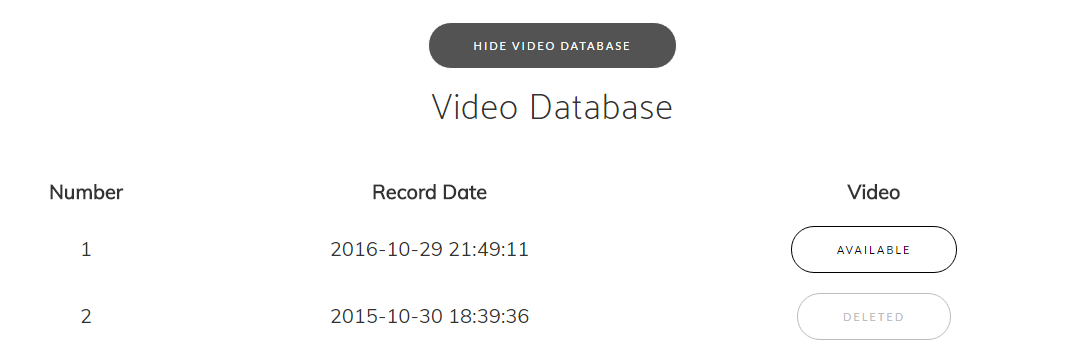
\includegraphics[width=1.0\textwidth]{images/phptable}
    \caption{Ausgabe der Video Database im Browser.}
\end{figure}
\\
Die Eintr\"age innerhalb der Tabelle, in der Spalte Video verweisen jeweils auf das Video, das unterhalb der Tabelle in die Seite eingebettet ist. So ist es dem User m\"oglich sich einen \"Uberblick \"uber die vorhandenen Aufzeichnungen zu verschaffen und beim Klick auf den Available-Button in der Tabelle zum Video zu gelangen.
In der Tabelle werden zudem auch die Eintr\"age von Aufzeichnungen angezeigt, bei denen das Video-File bereits die festgelegte Zeit \"uberschritten hat und gel\"oscht wurde. \\
\\
\begin{figure}[htb]
  \centering
    
\includegraphics[width=1.0\textwidth]{images/phpdel}
    \caption{Button zum L\"oschen der Eintr\"age}
\end{figure}
\\
Wenn diese Eintr\"age nicht mehr ben\"otigt werden, kann der User unterhalb der Tabelle mit Klick auf einen Button alle alten Eintr\"age aus der Datenbank l\"oschen lassen. Hierbei wird f\"ur jeden Eintrag, der kein VideoPath Eintrag in der Datenbank besitzt, ein SQL Befehl von dem PHP-Skript an den MySQL-Server gesendet, der diesen Eintrag l\"oscht.\\
\begin{figure}[htb]
  \centering
    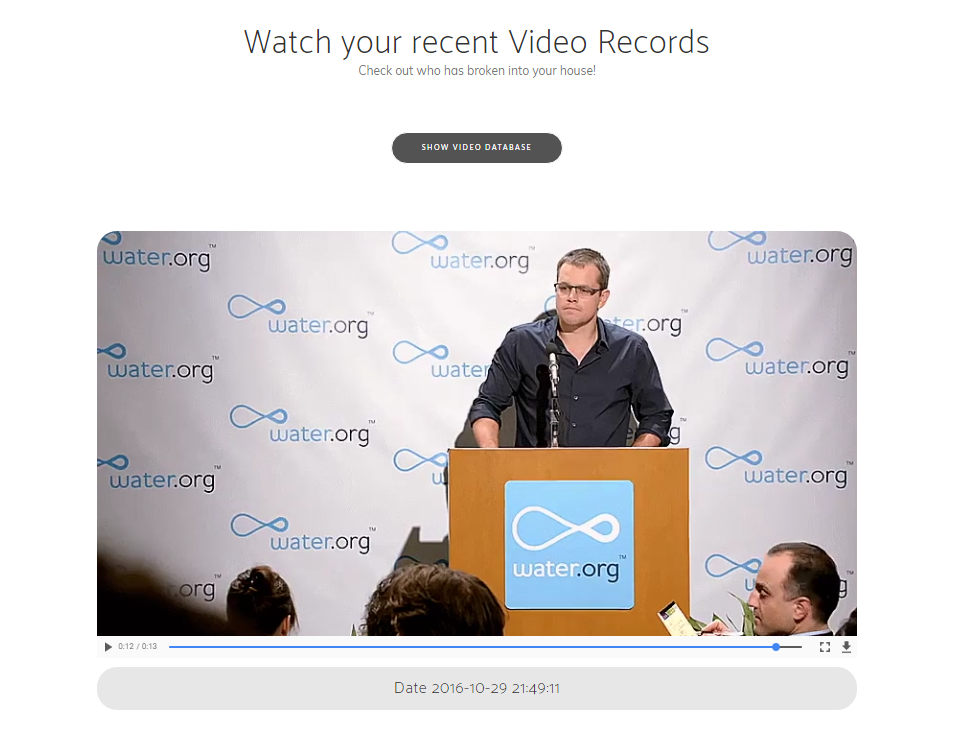
\includegraphics[width=1.0\textwidth]{images/video}
    \caption{Eingebettetes Video}
\end{figure}
\\
Unter der Tabelle der Video Database werden alle aufgezeichneten Videos mit Datum aufgelistet. Dabei fordert das PHP-Skript alle Eintr\"age aus der Records Tabelle an und iteriert in einer Schleife durch jeden Eintrag. Bei allen Eintr\"agen mit VideoPath Eintrag wird eine HTML Section\footnote{\hyperlink{https://developer.mozilla.org/de/docs/Web/HTML/Element/section}{https://developer.mozilla.org/de/docs/Web/HTML/Element/section}} generiert, in die das Video mittels Video-Tag eingebettet wird. Durch das Anlegen des Section-Tags ist es sp\"ater m\"oglich, den User zum entsprechenden Video zu schicken, nachdem er auf einen Eintrag in der Video Database Tabelle geklickt hat.\\


\begin{lstlisting}[language=PHP,caption={Auszug aus dem PHP-Skript (Videos auflisten)},numbers=left,frame=lrbt]
if ($result->num_rows > 0) 
{
    while($row = $result->fetch_assoc()) 
    {
        $i++;
		if($row["VideoPath"] != null)
		{	
			echo "<section id=\"" ."$i". "\">";			
			echo "<h2>";
			echo "
            <video width=\"100%\" height=\"auto\" controls>
                <source src=\" ". $row["VideoPath"]."\" type=\"video/mp4\">
                Your browser does not support the video tag.
            </video>";	
			echo "<h3>Date " . $row["RecordDateTime"]. "</h3><br><br>";		
			echo "</section>";
		}
    }
} 
\end{lstlisting}

\subsubsection{Frontend}

F\"ur das Webinterface wurde eine f\"ur das Projekt angepasste Version des Bootstrap\footnote{\hyperlink{http://getbootstrap.com/}{http://getbootstrap.com}} Theme New-Age\footnote{\hyperlink{https://startbootstrap.com/template-overviews/new-age/}{https://startbootstrap.com/template-overviews/new-age}} verwendet. Das HTML/CSS\footnote{\hyperlink{https://www.w3.org/TR/CSS22/}{https://www.w3.org/TR/CSS22}}/JS\footnote{\hyperlink{https://developer.mozilla.org/de/docs/Web/JavaScript}{https://developer.mozilla.org/de/docs/Web/JavaScript}} Framework Bootstrap besteht nur aus Clientseitigem Code und bietet daher wenig Fl\"ache f\"ur Angreifer. Es ben\"otigt wenig Ressourcen und verwendet den aktuellen Webstandard HTML 5.\\
\\
Die Anforderung war, dass das Frontend der Seite auf aktuellem HTML 5 aufbaut, light-weight\footnote{\hyperlink{http://whatis.techtarget.com/definition/lightweight}{http://whatis.techtarget.com/definition/lightweight}} ist d.h. wenig Server Ressourcen belegt und Angreifern wenig Spielraum l\"asst. Zudem muss sich das PHP-Skript einbetten lassen. Ein CMS\footnote{\hyperlink{https://de.wikipedia.org/wiki/Content-Management-System}{https://de.wikipedia.org/wiki/Content-Management-System}} wie z.B. Joomla\footnote{\hyperlink{https://www.joomla.org}{https://www.joomla.org}} ist hier zu anf\"allig f\"ur Angriffe\footnote{\hyperlink{https://www.heise.de/security/meldung/Jetzt-patchen-Angriffe-auf-ueber-30-000-Joomla-Webseiten-3454720.html}{https://www.heise.de/security/meldung/Jetzt-patchen-Angriffe-auf-ueber-30-000-Joomla-Webseiten-3454720.html}} und belegt unn\"otig Ressourcen. Daher wurde das light-weight CMS GRAV\footnote{\hyperlink{https://getgrav.org/}{https://getgrav.org}} in Betracht gezogen, das jedoch keine Einbindungen von PHP-Skripten unterst\"utzt. \\

\paragraph{Aufbau der Website}


\begin{figure}[htb]
  \centering
    
\includegraphics[width=1.0\textwidth]{images/webmenu}
    \caption{Men\"u des Webinterfaces}
\end{figure}

\begin{description}
   \begin{itemize}
      \item Intro mit allgemeinen Informationen.
      \item Download des Projekts von Github.
      \item Anzeige der Videoaufzeichnungen mittels PHP-Skript.
      \item Kontakt.
   \end{itemize}
\end{description}
\begin{figure}[htb]
  \centering
    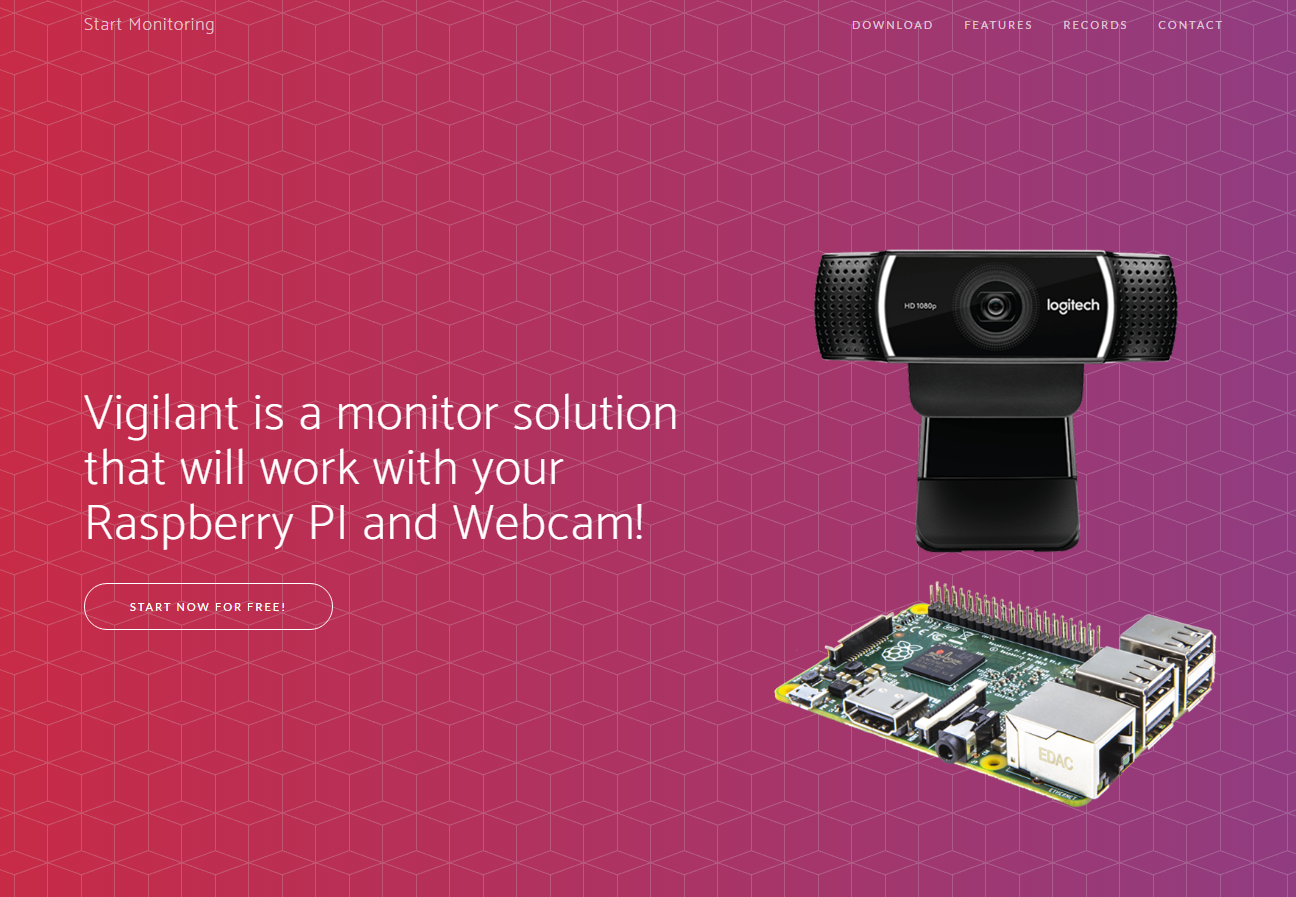
\includegraphics[width=1.0\textwidth]{images/vigilant}
    \caption{Intro der Projektseite}
\end{figure}
Eine exemplarische Implementierung findet man unter  {\href{https://www.schukies.io/vigilant}{https://schukies.io/vigilant}}









\chapter{Evaluation}

Im folgenden wird festgestellt, welche Projektziele erfolgreich umgesetzt wurden, und welche angepasst oder ausgeschlossen werden mussten.\\
\\
Das System zeichnet die Aufnahmen autonom auf. Der Magnetschalter wurde erfolgreich eingesetzt. Die Aufzeichnung beginnt kurz nach dem Betätigen des Magnet-Schalters.\\
Während die Tür offen ist, läuft die Aufnahme weiter. Wird die Tür geschlossen und innerhalb der Nachlaufzeit wieder geöffnet, läuft die Aufnahme weiter. Bleibt die Tür über die Nachlaufzeit geschlossen, wird die Aufnahme beendet.\\
Für jedes Öffnen der Tür wird ein Datenbank-Eintrag mit Datum, Uhrzeit und Video-Datei geschrieben. Videos, deren Alter eine bestimmte Anzahl an Tagen überschritten hat, werden gelöscht.\\
Über das Web-Interface lassen sich alle Einträge mit zugehörigem Video(falls vorhanden) anzeigen. Es wird außerdem eine Option zum Löschen der alten Einträge (Einträge ohne Video) bereitgestellt.\\
\\
Das Web-Interface wurde zudem in eine Projekt-Website eingebettet. Die Projekt-Website kann zur Demonstration im Internet veröffentlicht werden.

\vspace{1.0cm}

\section{Fazit}

Alle Projektziele wurden erfolgreich umgesetzt.\\
\\
Durch das Projekt wurde gezeigt, dass es möglich ist, Videoüberwachung eines oder mehrerer Gebäude-Zugänge kostengünstig und mit wenig Aufwand zu realisieren.\\
Mögliche Einsatz-Szenarien sind letztendlich abhängig von der Robustheit der Hardware-Installation; der entwickelte Prototyp dient zu Deonstrations-Zwecken und wurde in dieser Absicht angefertigt.\\
\\
Die Zusatzpunkte aus \ref{sec:kann} wurden für nicht ausschlaggebend befunden und daher weggelassen.

\vspace{1.0cm}

\section{Ausblick}

Das Projekt wird über Github anderen Entwicklern zur Verfügung gestellt. Zudem gibt es eine Website\footnote{\href{https://schukies.io}{schukies.io/vigilant}} zur Veranschaulichung mit einer Demo des Webinterfaces. Somit könnte es in Zukunft andere Projekte geben, die auf diesem aufbauen oder es erweitern.
\chapter{Anhang}

\section{Quellcode}

\lstinputlisting[language=SQL, numbers=left, frame=lrbt, caption={dbRecords.sql}]{work-done/source/dbRecords.sql}

\vspace{0.5cm}

\lstinputlisting[language=SQL, numbers=left, frame=lrbt, caption={dbUser.sql}]{work-done/source/dbUser.sql}

\newpage

\lstinputlisting[language={[5.1]Lua}, breaklines=true, numbers=left, frame=lrbt, caption={config.lua}]{work-done/source/config.lua}
\vspace{0.5cm}

\lstinputlisting[language={[5.1]Lua}, breaklines=true, numbers=left, frame=lrbt, caption={init.lua}]{work-done/source/init.lua}
\vspace{0.5cm}

\newpage

\lstinputlisting[language={[5.1]Lua}, breaklines=true, numbers=left, frame=lrbt, caption={record.lua}]{work-done/source/record.lua}
\vspace{0.5cm}

\newpage

\lstinputlisting[language={[5.1]Lua}, breaklines=true, numbers=left, frame=lrbt, caption={dbclean.lua}]{work-done/source/dbclean.lua}

\newpage

\lstinputlisting[breaklines=true, numbers=left, frame=lrbt, caption={dbclean.service}]{work-done/source/dbclean.service}
\vspace{0.5cm}

\lstinputlisting[breaklines=true, numbers=left, frame=lrbt, caption={dbclean.timer}]{work-done/source/dbclean.timer}
\vspace{0.5cm}

\lstinputlisting[breaklines=true, numbers=left, frame=lrbt, caption={record.service}]{work-done/source/record.service}

\newpage

\lstinputlisting[language=PHP, breaklines=true, numbers=left, frame=lrbt, caption={vigilant.php}]{work-done/source/vigilant.php}

\newpage
\cleardoublepage
%\pagebreak
\phantomsection
\addcontentsline{toc}{chapter}{Quellenverzeichnis}
\begin{thebibliography}{99}


\bibitem[IMG01]{img01}\url{https://cdn.sparkfun.com//assets/parts/7/4/9/7/11546-04.jpg}

\bibitem[IMG02]{img02}\url{https://assets.logitech.com/assets/54515/2/hd-webcam-pro-c920-gallery.png}

\bibitem[IMG03]{img03}\url{https://img.conrad.de/medias/global/ce/9000_9999/9500/9530/9539/1462834_LB_00_FB.EPS.jpg}

\bibitem[IMG04]{img04}\url{http://www.conrad.com/medias/global/ce/5000_5999/5900/5940/5943/1205899_BB_00_FB.EPS_1000.jpg}

\bibitem[IMG05]{img05}\url{https://cdn-reichelt.de/bilder/web/artikel_ws/C300/MAGNET_M4.jpg}

\end{thebibliography}

\listoffigures

\end{document}
